%!TEX root = ../thesis.tex
%*******************************************************************************
%****************************** Fourth Chapter *********************************
%*******************************************************************************

\chapter{Methodology}
\label{chapter5}

% **************************** Define Graphics Path **************************
\ifpdf
\graphicspath{{Chapter5/Figs/Raster/}{Chapter5/Figs/PDF/}{Chapter5/Figs/}}
\else
\graphicspath{{Chapter5/Figs/Vector/}{Chapter5/Figs/}}
\fi

\section{Monte Carlo Importance Sampling}
\label{sec:Impl-MCIP}
The most common application of Monte Carlo methods is evaluation of integrals in high dimensional space. There MC has a distinct advantage over quadrature methods, as the statistical error decreases with the square root of samples irregardless of the dimensionality of the problem. Integrals of a function $g(\mathbf{R})$
\begin{equation}
	I=\int g(\mathbf{R}) \mathrm{d} \mathbf{R},
\end{equation}
where $\mathbf{R}$ is the \emph{configuration} of the system or simply a \emph{walker}, can be integrated by use of an \emph{importance function} $\mathrm{P}(\mathbf{R})$, where $\int d \mathbf{R} \text{P}(\mathbf{R})=1$ and $\mathrm{P} (\mathbf{R}) \geq 0$. The integral can be rewritten in the form
\begin{equation}
	\int g(\mathbf{R}) \mathrm{d} \mathbf{R} = \int \frac{g(\mathbf{R})}{\mathrm{P}(\mathbf{R})} \mathrm{P}(\mathbf{R}) \mathrm{d} \mathbf{R} = \int f(\mathbf{R})\mathrm{P}(\mathbf{R}) \mathrm{d} \mathbf{R},
\end{equation}
where $f(\mathbf{R}) = g(\mathbf{R}) / \mathrm{P}(\mathbf{R})$.
The importance function $\mathrm{P}(\mathbf{R})$ can be interpreted as a probability density. If we generate an infinite number of random uncorrelated configurations $\mathbf{R}_m$ from the distribution $\mathrm{P}(\mathbf{R})$, the sample average is a good estimator of the integral $I$
\begin{equation}
	I=\lim _{M \rightarrow \infty}\left\{\frac{1}{M} \sum_{m=1}^{M} f\left(\mathbf{R}_{m}\right)\right\},
\end{equation}
and for an approximation with a finite number of samples
\begin{equation}
	I \approx \frac{1}{M} \sum_{m=1}^{M} f\left(\mathbf{R}_{m}\right).
\end{equation}
Under conditions where the central limit theorem holds~\cite{foulkes2001quantum}, the estimator is normally distributed with variance $\sigma_{f}^{2}/M$, which can also be estimated from the samples as
\begin{equation}
	\frac{\sigma_{f}^{2}}{M} \approx \frac{1}{M(M-1)} \sum_{m=1}^{M}\left[f\left(\mathbf{R}_{m}\right)-\frac{1}{M} \sum_{n=1}^{M} f\left(\mathbf{R}_{n}\right)\right]^{2}.
\end{equation}


\section{Metropolis-Hastings Algorithm}
\label{sec:Impl-MCMC}
The integration technique from the previous section relies on our ability to obtain samples from a probability distribution $\mathrm{P}(\mathbf{R})$. In the case of QMC these distributions are high-dimensional and cannot be directly sampled from. Moreover their normalisations are usually not known. 
The Metropolis-Hastings algorithm~\cite{hastings1970monte}, see Algorithm~1, avoids direct sampling from the distribution $\mathrm{P}(\mathbf{R})$ and is insensitive to its normalisation. It uses a Markov process whose stationary distribution $\pi(\mathbf{R})$ is the same as $\mathrm{P}(\mathbf{R})$	
to generate a sequence of configurations $\left\{\mathbf{R}_n\right\}_\mathrm{P}$ 
that are drawn from $\mathrm{P}(\mathbf{R})$. A Markov process is completely defined with its transition probability $\mathrm{P}(\mathbf{R} \rightarrow \mathbf{R}^\prime)$, which is the probability of transitioning from state $\mathbf{R}$ to state $\mathbf{R}^\prime$. For the process to have a unique stationary distribution two conditions must be met, the process must be \emph{ergodic} and it must obey \emph{detailed balance}
\begin{equation}
	\mathrm{P}(\mathbf{R}) \mathrm P(\mathbf{R} \rightarrow \mathbf{R}^\prime) = \mathrm{P}(\mathbf{R}^\prime) \mathrm P(\mathbf{R}^\prime \rightarrow \mathbf{R}),
\end{equation}
rewritten as
\begin{equation}
	\label{eq:detailed_balance}
	\frac{\mathrm P ({\mathbf{R}})}{\mathrm P ({\mathbf{R}^\prime})} = \frac{\mathrm P(\mathbf{R}^\prime \rightarrow \mathbf{R})}{\mathrm P(\mathbf{R} \rightarrow \mathbf{R}^\prime)}.
\end{equation}
The right transition probability $\mathrm P(\mathbf{R} \rightarrow \mathbf{R}^\prime)$ is not known, but we can express it with a trial move transition probability $\mathrm{T}(\mathbf{R} \rightarrow \mathbf{R}^\prime)$ which we sample and acceptance probability $\mathrm{A}(\mathbf{R} \rightarrow \mathbf{R}^\prime)$ as
\begin{equation}
	\mathrm P(\mathbf{R} \rightarrow \mathbf{R}^\prime) = \mathrm T(\mathbf{R} \rightarrow \mathbf{R}^\prime) \mathrm A(\mathbf{R} \rightarrow \mathbf{R}^\prime).
\end{equation}
For equation~\eqref{eq:detailed_balance} to hold, the acceptance probability must be 
\begin{equation}
	A\left(\mathbf{R} \rightarrow \mathbf{R}^{\prime}\right)=\min \left(1, \frac{\mathrm{T}\left(\mathbf{R}^{\prime} \rightarrow \mathbf{R}\right) \mathrm{P}\left(\mathbf{R}^{\prime}\right)}{\mathrm{T}\left(\mathbf{R} \rightarrow \mathbf{R}^{\prime}\right) \mathrm{P}(\mathbf{R})}\right).
\end{equation}
Thus to sample from any probability distribution we need only have the ability to calculate probabilities $\mathrm P(\mathbf{R})$ and to sample from a trial transition probability $\mathrm T(\mathbf{R} \rightarrow \mathbf{R}^{\prime})$. The efficiency of the algorithm depends on the amount of trial moves that we reject. All trial moves would be accepted if $\mathrm{T}(\mathbf{R} \rightarrow \mathbf{R}^{\prime})= \mathrm{P}(\mathbf{R}^\prime)$, which would just mean sampling from $\mathrm P$ directly and is the very problem we are trying to solve with Metropolis-Hastings. 	
\begin{algorithm}
	\label{alg:MCMC}
	\SetAlgoLined
	\KwResult{A set of configurations $\left\{ \mathbf{R}_n \right\}_{\mathrm{P}}$ sampled from $\mathrm P$}
	Initialize walker at random configuration $\mathbf{R}$\;
	\While{no. samples less than $N$}{
		Generate new configuration $\mathbf{R}^\prime$ with transition probability $\mathrm{T}(\mathbf{R}\rightarrow\mathbf{R}^\prime)$\;
		
		Accept the move ($\mathbf{R} \rightarrow \mathbf{R}^\prime$) with probability $A\left(\mathbf{R} \rightarrow \mathbf{R}^{\prime}\right)=\min \left(1, \frac{\mathrm{T}\left(\mathbf{R}^{\prime} \rightarrow \mathbf{R}\right) \mathrm{P}\left(\mathbf{R}^{\prime}\right)}{\mathrm{T}\left(\mathbf{R} \rightarrow \mathbf{R}^{\prime}\right) \mathrm{P}(\mathbf{R})}\right)$\;
		
		Append $\mathbf{R}$ to the set of configuration;
	}
	\caption{Metropolis-Hastings}
\end{algorithm}

\section{Gradient based optimisation}
\label{sec:gbopt}

\subsection{Gradient estimation}
\label{subsec:gbopt-gest}

\begin{itemize}
	\item \textbf{TODO:} Rewrite with a more general tone, do not only talk about the ELBO. Still use Mohammeds review! It is very good.
\end{itemize}

In order to perform gradient descent on the ELBO objective, we need to be able to evaluate its gradients with respect to parameters $\boldsymbol{\theta}$ and $\boldsymbol{\phi}$. Taking the gradient w.r.t generative parameters $\boldsymbol{\theta}$ is straightforward, because we can change the order of the expectation operator and the gradient, leaving us with
\begin{equation}
	\begin{aligned} 
		\nabla_{\boldsymbol{\theta}} \mathcal{L}_{\boldsymbol{\theta}, \boldsymbol{\phi}}(\mathbf{x}) &=\nabla_{\boldsymbol{\theta}} 	\mathbb{E}_{q_{\boldsymbol{\phi}}(\mathbf{z} \mid \mathbf{x})}\left[\log p_{\boldsymbol{\theta}}(\mathbf{x}, \mathbf{z})-\log q_{\boldsymbol{\phi}}(\mathbf{z} | \mathbf{x})\right] \\  & \simeq \nabla_{\boldsymbol{\theta}}\left(\log p_{\boldsymbol{\theta}}(\mathbf{x}, \mathbf{z})-\log q_{\boldsymbol{\phi}}(\mathbf{z} | \mathbf{x})\right) \\ &=\nabla_{\boldsymbol{\theta}}\left(\log p_{\boldsymbol{\theta}}(\mathbf{x}, \mathbf{z})\right) ,
	\end{aligned}
\end{equation}
where $\simeq$ denotes an unbiased estimator. This reversing of the order of operations is not possible when taking gradients w.r.t variational parameters $\boldsymbol{\phi}$ because the expectation $\mathbb{E}_{q_{\boldsymbol{\phi}}(\mathbf{z} | \mathbf{x})}$ is performed w.r.t the approximate posterior $q_{\boldsymbol{\phi}}(\mathbf{z} | \mathbf{x})$. The gradient could be estimated with a vanilla Monte Carlo estimator, but it has very high variance and is not practical~\cite{kingma2013auto}. 

The problem of stochastic gradient estimation of an expectation of a function is a well studied problem that transcends machine learning and has a variety of applications~\cite{chriss1997black, schrittwieser2020mastering}. Different estimators differ in from and their properties, variance being one of the most important. In their review~\cite{mohamed2020monte} Mohamed et al. categorise MC gradient estimators into three categories

\subsubsection{Score-function estimator}
\emph{Score-function estimator}: The score function is a logarithm of a probability distribution w.r.t to distributional parameters. It can be used as a gradient estimator
\begin{equation}
	\begin{aligned}
		\nabla_{\boldsymbol{\theta}} \mathbb{E}_{p_{\boldsymbol{\theta}}(\mathbf{x})}[f(\mathbf{x})] &=  \nabla_{\boldsymbol{\theta}} \int p_{\boldsymbol{\theta}}(\mathbf{x}) f(\mathbf{x}) d \mathbf{x} \\
		&= \mathbb{E}_{p_{\boldsymbol{\theta}}(\mathbf{x})}\left[f(\mathbf{x}) \nabla_{\boldsymbol{\theta}} \log p_{\boldsymbol{\theta}}(\mathbf{x})\right].
	\end{aligned}
\end{equation}
The score-function estimator is compatible with any cost function, it requires that the measure $p_{\boldsymbol{\theta}}(\mathbf{x})$ is differentiable and easy to sample. Very importantly it is applicable to both discrete and continuous distribution, but has a drawback of having high variance.

\subsubsection{Pathwise estimator}
Continuous distributions can be sampled either directly by generating samples from the distribution $p_{\boldsymbol{\theta}}(\mathbf{x})$ or indirectly, by sampling from a simpler base distribution $p(\boldsymbol{\epsilon})$ and transforming the variate through a deterministic path $g_{\boldsymbol{\theta}}(\boldsymbol{\epsilon})$. Using this, it is possible to move the source of randomness in such a way that the objective is differentiable. In essence this approach pushes the parameters of the measure into the cost function which is then differentiated. The estimator is
\begin{equation}
	\begin{aligned}
		\nabla_{\boldsymbol{\theta}} \mathbb{E}_{p_{\boldsymbol{\theta}}(\mathbf{x})}[f(\mathbf{x})] 
		&=\nabla_{\boldsymbol{\theta}} \int p_{\boldsymbol{\theta}}(\mathbf{x}) f(\mathbf{x}) d \mathbf{x} \\
		&= \nabla_{\boldsymbol{\theta}} \int p(\boldsymbol{\epsilon}) f(g_{\boldsymbol{\theta}}(\boldsymbol{\epsilon})) d \boldsymbol{\epsilon} \\
		&= \mathbb{E}_{p(\boldsymbol{\epsilon})}\left[\nabla_{\boldsymbol{\theta}} f(g_{\boldsymbol{\theta}}(\boldsymbol{\epsilon}))\right].
	\end{aligned}
\end{equation}
\begin{figure}
	\centering
	\subfloat[Original]{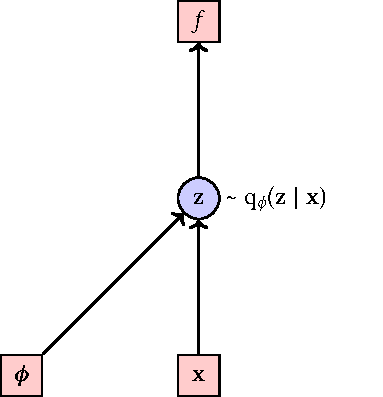
\includegraphics[height=7cm]{Appendix2/Figs/Vector/reparam_diagram.pdf}}
	\subfloat[Reparametrized]{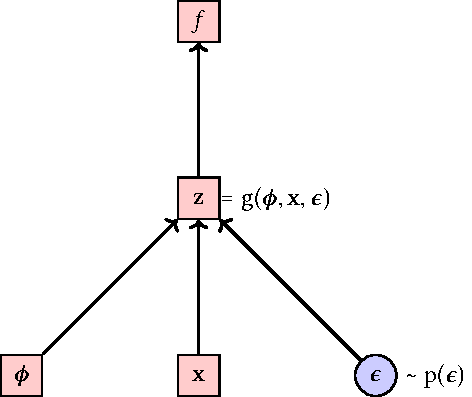
\includegraphics[height=7cm]{Appendix2/Figs/Vector/reparam_diagram2.pdf}}
	\caption[The reparametrization trick]{The reparametrization trick, adapted from~\cite{kingma2017variational}. The stochasticity of the $\mathbf{z}$ node is pushed out into a separate input to the same node, resulting in deterministic gradients w.r.t $\boldsymbol{\phi}$ through the node.}
	\label{fig:reparam}
\end{figure}
This was the gradient estimator originally used in the VAE implementation~\cite{kingma2013auto} there named as the \emph{reparametrization trick}, see also Figure~\ref{fig:reparam}. In many cases the transformation paths are so simple they can be implemented in one line of code, referred to as \emph{one-liners}. The pathwise-estimator can only be used on differentiable cost functions, but is easy to implement and crucially has lower variance than the score-function estimator. 

\subsubsection{Measure-valued gradient estimator}
Which exploits the properties of signed-measures, is beyond the scope of this report.	

\subsection{Automatic differentiation}
\label{subsec:gbopt-autograd}

\section[\emph{Qptimal sampling}]{\emph{Qptimal sampling}: optimal sampling in lattice models}